
\begin{document}
\title{COMS3008A Assignment -- Report}
\author{Claudio Da Mata - 2128358}
\date{23-10-2022} 
\maketitle 
%\thispagestyle{empty}
\pagestyle{fancy}
\fancyhf{}
\fancyhead[R]{\thepage}
\fancyhead[L]{COMS3008A Assinment}
%\vskip 3mm 
%\pagenumbering{roman}
%\newpage
\pagenumbering{arabic} 
\section{Problem 1: Parallel Scan}
\begin{itemize}
	\item  Given a set of elements, $[a_0,a_1,\dotsm,a_{n-1}]$, the scan operation associated with addition operator for this input is the output set $[a_0,(a_0+a_1),\dotsm,(a_0+a_1+\dotsm+a_{n-1})]$. 
	\item For example, the input set is $[2,1,4,0,3,7,6,3]$, then the scan with addition operator of this input is $[2,3,7,7,10,17,23,26]$. 
\end{itemize}
\subsection{Serial Implementation:}
Firstly I started off with the baseline implementation of serial scan operation.
\begin{lstlisting}[caption=Sequential algorithm for computing scan operation with ‘+’ operator]
	void scan(int out[], int in[], int N){
		out[0] = in[0];
		
		for(int i=1; i<N; i++) {
			out[i] = in[i] + out[i-1];
		}
	}
\end{lstlisting}

\section{Problem 2: Parallel Bitonic Sort}
The bitonic sort is based on the idea of sorting network. The bitonic sorting algorithm is suitable for parallel processing, especially for GPU sorting. \textbf{However, in this problem, you are requested to implement parallel bitonic sorting of integers using \textbf{OpenMP and MPI}, respectively. }

Another paragraph starts \dots
\section{Problem 3: Parallel Graph Algorithm}
An example figure is given in Figure~\ref{fig:sp_fig1}.
\begin{figure}[htb]
	\centering
	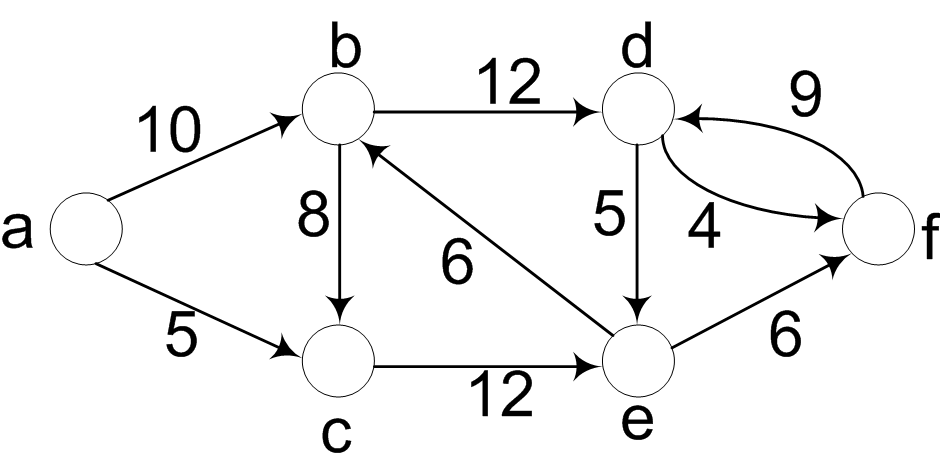
\includegraphics[width=0.5\linewidth]{pics/sp_fig1.png}
	\caption{A directed graph}\label{fig:sp_fig1}
\end{figure}

An example of table is given Table~\ref{tab:example}.
\begin{table}[htb]
	\centering
	\caption{An example of a table}\label{tab:example}
	\begin{tabular}{l|ccccc}
		\toprule
		No of vertices & 64 & 128 & 256 & 384 & 512\\
		\midrule
		Serial &0.1&0.2&0.3&0.4&0.5\\
		Parallel &&&&\\
		Sppedup &2&3&4&5&6\\
		\bottomrule
	\end{tabular}
\end{table} 

\end{document} 

